\documentclass[aps,prl,twocolumn,superscriptaddress]{revtex4-1}

\usepackage{graphicx,bm,multirow,amssymb,amsmath,xcolor,soul}

\begin{document}

\title{Towards predictive many-body calculations of phonon-limited carrier mobilities in semiconductors\\[6pt]
Supplemental Material}

\author{Samuel Ponc\'e}
\affiliation{Department of Materials, University of Oxford, Parks Road, Oxford, OX1 3PH, UK}
\author{Elena R. Margine}
\affiliation{Department of Physics, Binghamton University-SUNY, Binghamton, New York 13902, USA}
\author{Feliciano Giustino}
\email{feliciano.giustino@materials.ox.ac.uk}
\affiliation{Department of Materials, University of Oxford, Parks Road, Oxford, OX1 3PH, UK}

\newcommand{\mobun}{{cm$^2$/Vs}}
\renewcommand{\thetable}{S\arabic{table}}
\renewcommand{\thefigure}{S\arabic{figure}}
\def\a{{\alpha}}
\def\b{{\beta}}
\def\ve{{\varepsilon}}
\def\w{\omega}
\def\bk{{\bf k}}
\def\bq{{\bf q}}
\def\bG{{\bf G}}
\def\d{\delta}
\def\>{\rangle}
\def\<{\langle}
\def\D{\partial}
\def\kt{k_{\rm B}T}
\def\hbp{{\hat{\bf p}}}

\date{\today}

\maketitle

\subsection{Computational Methods}

In this work we use norm-conserving pseudopotentials with planewave kinetic energy cutoffs of 45~Ry 
and 35~Ry for LDA and PBE calculations, respectively. The phonon dispersion relations are evaluated
using density-functional perturbation theory~\cite{Baroni2001}, starting from a 
6$\times$6$\times$6 uniform grid of $\bq$-points. An 18$\times$18$\times$18 uniform grid of $\bk$-points 
was required to correctly obtain vanishing Born effective charges.
Representative phonon dispersion relations obtained
within this setup can be found in Ref.~\cite{Ponce2016a}. 
The coarse grids for the electron-phonon interpolation required 12$\times$12$\times$12 $\bk$-points and 
6$\times$6$\times$6 $\bq$-points. Such a dense $\bk$-grid was needed to obtain a good Wannier interpolation
of the conduction bands, since the minimum is along the $\Delta$ line (approx.~0.85$\Gamma$X) 
and does not fall on a high-symmetry point.  


For the self-consistent, iterative solution of the Boltzmann transport equation (IBTE) we employ
uniform Brillouin-zone grids, and the $\bq$-point sums are restricted to the irreducible wedge
of the Brillouin zone using crystal symmetry operations. The IBTE is solved using homogeneous and commensurate
$\bk$- and $\bq$-point grids since the variations $\D_{E_\b} f_{n\bk}^{i+1}$ at the $(i+1)$-th
iteration require the knowledge of the variations $\D_{E_\b} f_{n\bk+\bq}^{i}$ at the $i$-th iteration,
see Eq.~(2) of the main text.

For the direct solution of the BTE within the self-energy relaxation time approximation (SERTA)
the Brillouin zone grids do not need to be commensurate. In this case, in order to improve the sampling 
accuracy, we employ quasi-random Sobol sequences of $\bk$- and $\bq$-points. Following recommended
practice, we skip the first 1000 elements of a sequence and we retain one element every 100 of the
remainder~\cite{Bratley1988}; furthermore we employ a linear scramble and shift of the resulting
sequence, using standard routines from \texttt{Matlab~R2015a}~\cite{Hong2003}. As a further
refinement we replace the homogeneous Sobol weights using a Voronoi
triangulation with the code \texttt{Voro++}~\cite{Rycroft2009}. In the Voronoi triangulation we take
into account the periodicity of the Brillouin zone by building periodic replicas of the random grid
in neighboring reciprocal unit cells. For the $\bk$-point grid we also densify the distribution
around the band extrema, in order to capture the fine features of the scattering near the band edges.
This is achieved by generating additional random points with the Lorentz distribution
$1/(1+|\bk-\bk_0|^2/\gamma^2)$ and by recomputing the Voronoi weights of the resulting grid. Here $\bk_0$ indicates the location of the band extrema and $\gamma=0.008$~\AA$^{-1}$.


\begin{figure}
  \centering
  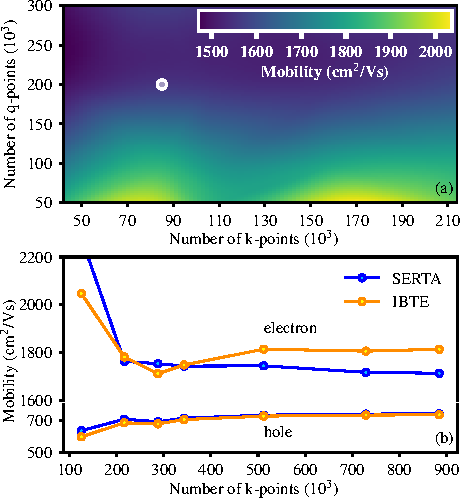
\includegraphics[width=\columnwidth]{figS1.pdf}  
  \caption{\label{fig1}
  (a) Sensitivity of the intrinsic electron mobility of silicon at 300~K with respect to the sampling 
  of electron ($\bk$) and phonon ($\bq$) wavevectors in the Brillouin zone. The calculations are
  performed within the SERTA approximation, using a densified Lorentzian distribution of $\bk$-points around 
  the conduction band minima, and a Sobol quasi-random sampling of the $\bq$-points. The white dot
  indicates the setup used in the calculations reported in the main text of this article.
  (b) Comparison between the rate of convergence of the intrinsic electron and hole mobilities of silicon 
  using the SERTA and the IBTE approaches, at 300~K. In this case we use uniform grids, with the $\bk$-point
  mesh being twice as dense as the $\bq$-point mesh in each direction.
  }
\end{figure}

Figure~\ref{fig1}(a) shows the convergence of the intrinsic mobility of silicon at 300~K with respect to
the number of electron and phonon wavevectors in the Brillouin zone within the SERTA approximation. 
Figure~\ref{fig1}(b) shows the comparison between calculations of the intrinsic mobility of silicon within the SERTA and the IBTE approaches.

The GW calculations are performed starting from the PBE band structure and using the experimental
lattice parameters on a 12$\times$12$\times$12 $\bk$-point grid. To obtain direct and indirect band gaps converged to within 5~meV
we use 120~bands and a planwaves cutoff of 15~Ry for the dielectric matrix. The renormalization
of the band velocity is evaluated as in Ref.~\cite{Rohlfing2000}: 
$\< \psi_{n\bk} | \hbp | \psi_{m\bk}\>_{\rm GW} = 
[(\ve_{n\bk}^{\rm GW}-\ve_{m\bk}^{\rm GW})/(\ve_{n\bk}^{\rm DFT}-\ve_{m\bk}^{\rm DFT})]
\< \psi_{n\bk} | \hbp | \psi_{m\bk}\>_{\rm DFT}$, where $\hbp$ indicates the momentum operator.
When $n=m$ the previous expression is replaced by 
$\< \psi_{n\bk} | \hbp | \psi_{n\bk}\>_{\rm GW} = \< \psi_{n\bk} | \hbp | \psi_{n\bk}\>_{\rm DFT}$.


For completeness the effective masses computed within scalar-relativistic DFT, fully-relativistic DFT,
and including GW quasiparticle corrections are reported in Table~\ref{table1}. 
We also show in Table~\ref{table2} the effective masses calculated without SOC at the experimental lattice parameter with 
two different types of pseudization (norm-conserving and ultrasoft), and two exchange and correlation 
functionals (LDA and PBE). 


In order to calculate mobilities using band structures as close as possible to experiments
(i.e. the lowermost bars in Fig.~1),
we repeated the calculations using the low-energy dispersion relations parametrized 
in Refs.~\onlinecite{Dresselhaus1955,Yu2010} starting from the measured effective masses:
\begin{align}
\varepsilon_{\text{cb}} =& \frac{\hbar^{2}(k_x-k_{0,x})^2}{2m_{||}}+ \frac{\hbar^{2}(k_y-k_{0,y})^2}{2m_{\perp}} \nonumber\\
                        &  + \frac{\hbar^{2}(k_z-k_{0,z})^2}{2m_{\perp}} + \varepsilon_{\rm c}, \\
\varepsilon_{\text{hh}} =& Ak^2 + [B^2k^4 + C^2(k_x^2k_y^2 + k_y^2k_z^2 + k_z^2k_x^2)]^{1/2},\\
\varepsilon_{\text{lh}} =& Ak^2 - [B^2k^4 + C^2(k_x^2k_y^2 + k_y^2k_z^2 + k_z^2k_x^2)]^{1/2},\\
\varepsilon_{\text{so}} =& -\frac{k^2\hbar^2}{2m_{\text{so}}} - \varepsilon_{\text{so}},
\end{align}
where $m_{||}=0.98m_0$ ($m_0$ is the free electron mass), 
$m_{\perp}=0.19m_0$, $m_{\text{so}}=0.23m_0$,  $\bk_0$ denotes the wavevectors of 
the conduction band minima, and $\varepsilon_{\rm c}$ is the conduction band bottom. 
The coefficients are $A=-4.1\,\hbar^2/2m_0$, $B=-1.6\,\hbar^2/2m_0$ 
and $C=3.3\,\hbar^2/2m_0$~\cite{Dresselhaus1955,Yu2010} and 
$\varepsilon_{\text{so}}$ = 48~meV.


\begin{table}
  \begin{tabular}{c c c c c c }
  \toprule
  Band & Direction & \multicolumn{3}{c}{Present calculations} & Expt. \\
  \multicolumn{2}{c}{}   & No SOC & SOC & SOC+GW &     \\
  \hline\\[-8pt]
  \multirow{3}{*}{Split-off hole}
  & [100]                & 0.167  & 0.224 &  0.226 &  0.23  \\
  & [111]                & 0.094  & 0.227 &  0.227 &  0.23  \\
  & [110]                & 0.106  & 0.227 &  0.225 &  0.23  \\
  \multirow{3}{*}{Light hole}
  & [100]                & 0.253  & 0.189 &  0.202 &  0.17 \\
  & [111]                & 0.682  & 0.131 &  0.132 &  0.16 \\
  & [110]                & 0.266  & 0.140 &  0.140 &  0.16 \\
  \multirow{3}{*}{Heavy hole}
  & [100]                & 0.271  & 0.256 &  0.243 &  0.46 \\
  & [111]                & 0.694  & 0.654 &  0.643 &  0.56 \\
  & [110]                & 2.868  & 0.521 &  0.512 &  0.53 \\
  \multirow{2}{*}{Electron}  
          & long.  & 0.798  & 0.824 &  1.090  & 0.98 \\ 
          & trans. & 0.188  & 0.190 &  0.186  & 0.19 \\
  \botrule 
  \end{tabular}
  \caption{\label{table1}
  Comparison between calculated and measured effective masses of silicon, in units of the electron mass.
  The experimental data are from Refs.~\onlinecite{Dexter1954,Sze2007,Yu2010}.
  }
\end{table}


\begin{table}
  \begin{tabular}{c c c c c c }
  \toprule
  Band & Direction       & LDA-US       & LDA          & PBE        &  Expt. \\
  \hline\\[-8pt]
  \multirow{3}{*}{Split-off hole}
  & [100]                & 0.170 & 0.168 & 0.167  &   0.23  \\
  & [111]                & 0.098 & 0.098 & 0.094  &   0.23  \\
  & [110]                & 0.111 & 0.109 & 0.106  &   0.23  \\
  \multirow{3}{*}{Light hole}
  & [100]                & 0.248 & 0.265 & 0.253  &   0.17 \\
  & [111]                & 0.551 & 0.655 & 0.682  &   0.16 \\
  & [110]                & 0.271 & 0.278 & 0.266  &   0.16 \\
  \multirow{3}{*}{Heavy hole}
  & [100]                & 0.271 & 0.276 & 0.271  &   0.46 \\
  & [111]                & 0.635 & 0.678 & 0.694  &   0.56 \\
  & [110]                & 2.158 & 2.170 & 2.868  &   0.53 \\
  \multirow{2}{*}{Electron}  
          & long.  & 0.755 & 0.735 & 0.771  &   0.98 \\ 
          & trans. & 0.182 & 0.185 & 0.188  &   0.19 \\
  \botrule 
  \end{tabular}
  \caption{\label{table2}
  Comparison between effective masses calculated using different types of pseudopotentials and exchange-correlation functionals without SOC, in units of the electron mass.
  The experimental data are from Refs.~\onlinecite{Dexter1954,Sze2007,Yu2010}.
  }
\end{table}


%%%%%%%%%%%%%%%%%%%%%%%%%%%%%%%%


\subsection{Broadening of Dirac delta functions}
The numerical evaluation of phonon-limited mobilities using Eqs.~(2)-(4) of the main text requires one to
replace the Dirac delta functions in Eqs.~(2)-(3) by Lorentzian functions with finite broadening $\eta$: 
$\pi\,\d(\ve_{n\bk}\pm\hbar\w_{\bq\nu}-\ve_{m\bk+\bq}) \rightarrow {\rm Im}\,(\ve_{n\bk}\pm\hbar
\w_{\bq\nu}-\ve_{m\bk+\bq}-i\eta)^{-1}$. This procedure makes the calculated mobility dependent
on the broadening parameter, hence it is important to check how sensitive are the results to the 
choice of $\eta$.

Figure~\ref{figS2}(a) shows the intrinsic electron mobility of silicon at 0~K, evaluated as a function of $\eta$.
From this figure we see that the mobility tends to diverge towards $+\infty$ as $\eta\rightarrow 0$.
This trend can be rationalized by noting that the mobility is directly proportional to the relaxation
time [cf.\ Eq.~(5) of main text], and the relaxation time due to acoustic phonon scattering in a
non-polar semiconductor is inversely proportional to the temperature~\cite{Bardeen1950}. As a result, we expect that the phonon-limited
mobility will increase indefinitely as $\eta$ becomes smaller and the Lorentzian approaches the Dirac 
delta function. This observation is in agreement with the explicit calculations in Fig.~\ref{figS2}(a).

This behavior poses a problem when one has to decide which broadening parameter to use in the
calculations. As a general rule here we set $\eta$ to the smallest possible value where the
curve $\mu$ vs.\ $\eta$ is relatively flat, so that our results are insensitive to this choice.
Based on Fig.~\ref{figS2}(a), we use $\eta = 5$~meV in all calculations presented in the article. This choice
is consistent with the notion that real quasiparticles do not have an infinite lifetime as it is assumed 
in the BTE formalism, but have a finite lifetime due to electron-electron and electron-phonon interactions.
In Fig.~\ref{figS2}(b) we show our calculated quasiparticle broadening from electron-phonon interactions at
0~K and 300~K. It can be seen that at 300~K the broadening reaches values up to 4-5~meV 
for quasiparticle energies located one phonon energy away from the band bottom (the highest phonon
energy in silicon is $\sim$63~meV). These values are consistent with our choice of broadening parameter.

\begin{figure}
  \centering
  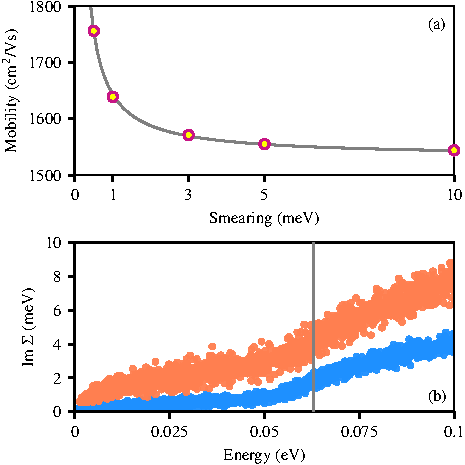
\includegraphics[width=\columnwidth]{figS2.pdf}
  \caption{\label{figS2}
  (a) Intrinsic electron mobility of silicon at 0~K, 
  calculated as a function of the broadening parameter $\eta$
  (dots). The grey thin line is a guide to the eye and was obtained by fitting the data points using
  $\mu = {\rm const}/ \eta$.
  (b) Electron quasiparticle linewidths in silicon arising from the electron-phonon interaction,
  calculated at 0~K (blue dots) and 300~K (orange dots). The zero of the horizontal energy axis is set
  to the conduction band minimum. The vertical grey line indicates the energy of the highest optical
  phonon in silicon.
  }
\end{figure}

\subsection{Screening of the electron-phonon matrix elements}

The strategy that we used to correct for the DFT overscreening of the electron-phonon matrix elements
consists of un-screening the matrix elements via the DFT dielectric function, so as to obtain
the bare matrix elements, and then screening the bare matrix elements using the best possible
dielectric function. The dielectric function can be factored out of the integral in the matrix element
if we neglect local field effects.
Since local field effects are known to decrease the head of the dielectric function of silicon by 10\%
and the body of the dielectric function 
is typically one or two orders of magnitude smaller than the head~\cite{Hybertsen1987}, we expect 
to make an error on the order of a few percent. 

In order to perform this operation for a large number of phonon wavevectors
we use the Thomas-Fermi model dielectric function of Ref.~\onlinecite{Resta1977}:
  \begin{equation}\label{eq.model}
  \epsilon(q) = \frac{k_0^2+q^2}{k_0^2 \sin (qR)/(qR\,\epsilon_0) + q^2 },
  \end{equation}
where $q=|\bq|$, $\epsilon_0$ is the macroscopic (electronic) dielectric constant. $k_0$ are $R$ are obtained from the valence electron density $\rho$ as 
$k_0^2 = 4(3\pi^2 \, \rho)^{1/3}/\pi$ and $\sinh (k_0R)/k_0R = \epsilon_0$. The only free parameter of the model is $\epsilon_0$. 

We test the validity of this model by computing the dielectric matrix within the random phase approximation (RPA),
using a 12$\times$12$\times$12 unshifted grid (corresponding to 72~inequivalent wavevectors).
Figure~\ref{figS3} shows a comparison between the model dielectric function of Eq.~\eqref{eq.model} 
and the RPA calculation,
after matching $\epsilon_0$ to the head of the RPA dielectric matrix. We see that Eq.~\eqref{eq.model} reproduces well the RPA
screening, therefore it is sensible to use it in the renormalization of the electron-phonon
matrix elements. In this work we renormalized the matrix elements by setting $\epsilon_0$ to the
experimental dielectric constant of silicon (11.94). 

\begin{figure}
  \centering
  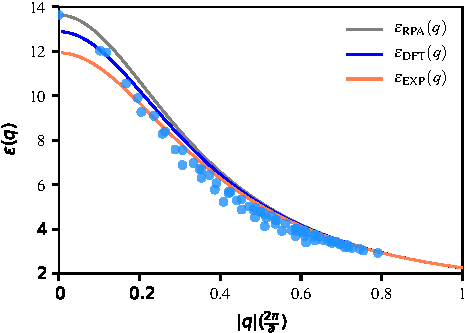
\includegraphics[width=\columnwidth]{figS3.pdf}
  \caption{\label{figS3}
  Comparison between the diagonal part of the RPA dielectric matrix of silicon (blue dots) and the Thomas-Fermi
  model of Ref.~\onlinecite{Resta1977} (grey line). 
  We also show the model dielectric function using the DFT dielectric constant $\varepsilon(0)=12.89$ (blue line) and 
  experimental dielectric constant $\varepsilon(0)=11.94$ (orange line).
  }
\end{figure}

\subsection{Brooks-Herring model for impurity scattering}

In order to account for impurity scattering in Fig.~3(b) of the main text, we use the
semi-empirical model developed by Brooks and Herring~\cite{Brooks1951,Li1977}.
In this model the mobility $\mu_{\rm i}$ is evaluated analytically by taking into
account quantum-mechanical scattering rates, spherical energy surfaces, negligible 
electron-electron interactions, and complete ionization of the impurities. 
The explicit expression of the hole mobility is:
  \begin{equation}\label{BHequation}
  \mu_{\rm i} = \frac{2^{7/2} \epsilon_s^2 (\kt)^{3/2} }{\pi^{3/2} e^3 \sqrt{m_d^*} \,n_{\rm i} 
  G(b)} \quad \bigg[\frac{\rm{cm^2}}{\rm{Vs}}\bigg],
  \end{equation}
where $G(b) = \ln(b+1) - b/(b+1)$, $b = 24\pi m_d^* \epsilon_s (\kt)^{2}/e^2 h^2 n'$, and
$n'=n_{\rm h}(2-n_{\rm h}/n_{\rm i})$.
Here $m_d^*=0.55 m_0$ is the density-of-state effective mass for the holes~\cite{Balkanski2000}, $n_{\rm h}$ and $n_{\rm i}$ are the hole densities and 
the density of ionized impurities [impurity concentration in Fig. 3(b) of the main text], 
respectively, $\epsilon_s=11.9\epsilon_0$ is the dielectric constant, $\epsilon_0$ is the
permittivity of vacuum, and $h$ is Planck's constant. In the above expressions, 
the concentrations are expressed in cm$^{-3}$, and the temperature $T$ is in K.

In the case of silicon, Eq.~\eqref{BHequation} cannot be used for the electron mobility 
because the electron mass is highly anisotropic and leads to incorrect results. To account for the electron mass 
anisotropy, we instead used the Long-Norton mobility expression~\cite{Norton1973,Li1977}:
  \begin{equation}
  \mu_{\rm i}^{\rm{LN}} = \frac{7.3\cdot 10^{17} T^{3/2} }{n_i G(b)} \quad \bigg[\frac{\rm{cm^2}}{\rm{Vs}}\bigg],
  \end{equation}
where the electron density-of-state effective mass is $m_d^*=1.08 m_0$~\cite{Sze2007}.

 Finally, the mobility including phonon ($\mu_l$) and impurity ($\mu_i$) scattering can be computed using the 
 mixed-scattering formula~\cite{Li1977}:
  \begin{equation}
  \mu =\mu_l \Big[ 1 + X^2\{ \text{ci}(X)\cos(X) + \sin(X)(\text{si}(X)-\frac{\pi}{2})\}  \Big], 
  \end{equation}
where $X^2 = 6\mu_l/\mu_i$ and ci(X) and si(X) are the cosine and sine integrals. 


\subsection{Effect of thermal lattice expansion}

Within the quasi-harmonic approximation~\cite{Baroni2010}, the Helmholtz free energy of a 
cubic crystal is given by~\cite{Palumbo2017}:
\begin{equation}
F(T,V) = U(V) + F^{\rm{vib}}(T,V) + F^{\rm{el}}(T,V),
\end{equation}
where $U$ is the static energy at 0~K, $F^{\rm{vib}}$ is the contribution due to lattice vibration 
and $F^{\rm{el}}$ the energy due to electronic thermal excitations. 
We rely on the adiabatic approximation to treat each term independently. 
The vibrational Helmholtz free energy per cell is given in the harmonic approximation by~\cite{Palumbo2017}: 
\begin{align}
F^{\rm{vib}}(T,V) =& \frac{1}{2N} \sum_{\mathbf{q},\nu} \hbar \omega_{\mathbf{q},\nu}(V) \nonumber \\
+& \frac{k_B T}{N}  \sum_{\mathbf{q},\nu} \ln \bigg[ 1 - \exp\Big( \frac{-\hbar \omega_{\mathbf{q},\nu}(V)}{k_B T} \Big) \bigg],
\end{align}
where $N$ is the number of $\bf q$-points, the first term is the contribution to the zero-point energy and the second term is the 
phonon contribution at finite temperature. $F^{\rm{el}}$ can be neglected as the band
gap is much larger than thermal energies.

The energy minimum of $U(V) + F^{\rm{vib}}(T,V)$ at a given temperature corresponds to zero pressure and gives the variation of volume
with temperature due to thermal expansion. 
To perform those calculations we used the \texttt{thermo\_pw} code~\cite{thermopw,Corso2016}.
The phonon frequencies were computed using the same LDA and PBE pseudopotentials as in the manuscript, without spin-orbit coupling, at nine different volumes. The resulting energies were fitted using the Murnaghan equation of state~\cite{Murnaghan1944}. 
We used a 18$\times$18$\times$18 $\mathbf{k}$-point grid for the electron and a 6$\times$6$\times$6 $\mathbf{q}$-point grid for the phonons. 
The obtained volume variation is given in Fig.~\ref{figS4}.

\begin{figure}
  \centering
  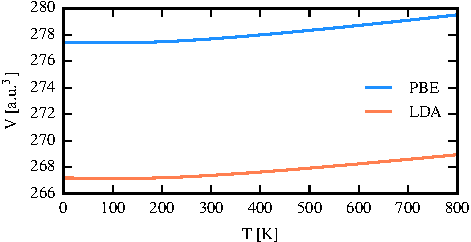
\includegraphics[width=\columnwidth]{figS4.pdf}
  \caption{\label{figS4}
  Variation of volume with temperature due to thermal expansion using the LDA or PBE exchange correlation functionals.
  }
\end{figure}


The change of eigenenergies due to thermal expansion is given by~\cite{Lautenschlager1985}:
\begin{equation}\label{renormeigen}
\Delta \varepsilon_{n\mathbf{k}} (T) = - \frac{\partial \varepsilon_{n\mathbf{k}}}{\partial P} \Big|_{T} \int_0^T dT' 3\alpha(T') B(T'),
\end{equation}
where $B(T) = -V(\partial P/\partial V)_T$ is the bulk modulus and $3\alpha = V^{-1}(\partial V/\partial T)_P$ is the 
thermal expansion coefficient. $B$ and $\alpha$ are obtained via numerical differentiation
starting from the volumes calculated in the above figure. 

We note that in Eq.~\ref{renormeigen} we carried the $\partial \varepsilon_{n\mathbf{k}}/\partial P$ term out of the temperature 
integral. This common temperature-independent approximation is valid in the elastic regime. 
To make sure that this approximation is valid, we compute $\partial \varepsilon_{n\mathbf{k}}/\partial P$ at 4~K and 300~K
by numerical derivation around the equilibrium volume for that temperature. From Table~\ref{tableS1}
 we see that indeed the temperature dependence is negligible and we therefore use the value at 4~K in Eq.~\ref{renormeigen}.

\begin{table}
  \begin{tabular}{l r r r r }
  \toprule
$\partial \varepsilon_{n\mathbf{k}}/\partial P$ & \multicolumn{2}{c}{LDA} & \multicolumn{2}{c}{PBE} \\
eV/Mbar                                         &   4 K       & 300 K     & 4 K       & 300 K \\
  \hline
%VBM     & 11.2573250666   &  11.2623783012  & 11.841529621       & 11.8745669506 \\
%CBM     &  9.53512857839  &  9.54115603027  &  9.85438063944     &  9.88407562831 \\
%Ind Gap & -1.72219648821  & -1.72122227093 & -1.98714898156 & -1.99049132229\\ 
VBM     & 11.257  &  11.262  & 11.841  & 11.874 \\
CBM     &  9.535  &   9.541  &  9.854  &  9.884 \\
Ind. Gap & -1.722  &  -1.721  & -1.987  & -1.990 \\ 
%Ind. Gap  exp.~\cite{Chang1984} &\multicolumn{4}{c}{-1.41, -1.5, -1.6, -3.8 }  \\
  \botrule 
  \end{tabular}
  \caption{\label{tableS1}
   Variation of the eigenenergies with pressure at two temperatures using the PBE and LDA pseudopotentials. %Experimental references are from Ref.~\onlinecite{Chang1984}.
  }
\end{table}

\begin{figure}
  \centering
  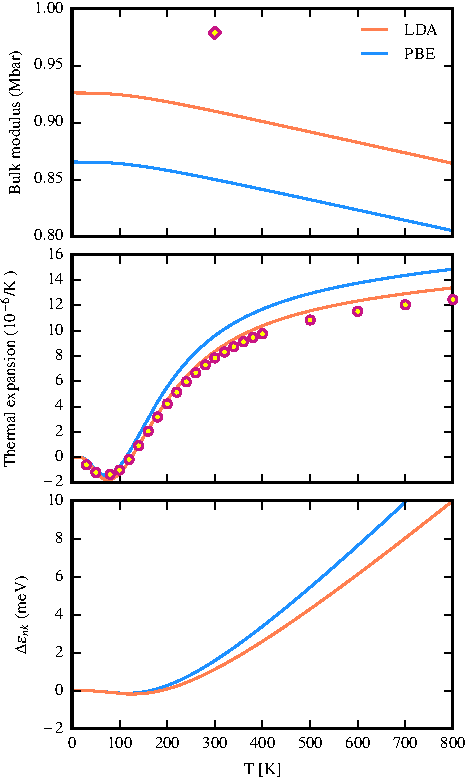
\includegraphics[width=\columnwidth]{figS5.pdf}
  \caption{\label{figS5}
   Variation of the bulk modulus, the thermal expansion and eigenstates renormalization with temperature of silicon.
   Experimental values are from Refs.~\onlinecite{McSkimin1964a} (yellow diamond) and \onlinecite{Okada1984} (yellow dots).
   %Prior LDA calculation is also reported from Ref.~\onlinecite{Rignanese1995} (yellow square).
  }
\end{figure}

The bulk modulus, the thermal expansion and eigenstates renormalization with temperature of silicon computed with the LDA and PBE exchange-correlation 
functionals are presented in Fig.~\ref{figS5}. 
From the bottom panel we see that thermal lattice expansion leads to a slight increase of the band gap 
of silicon. 
For PBE, the valence band top and conduction band bottom change by $-$9.5~meV and 
$-$7.8~meV from 0~K to 300~K, therefore the net increase of the band gap is 1.7~meV. This variation
is much smaller than the gap renormalization arising from electron-phonon interactions (as discussed
next), therefore in the present case this effect can safely be neglected when calculating
carrier mobilities.

\subsection{Electron-phonon renormalization of the bandstructures and free carrier screening}

The electron-phonon renormalization of the bandstructure has been discussed 
for the case of silicon in considerable detail in Ref.~\onlinecite{Ponce2015}.
The calculated zero-point renormalization of the
fundamental gap is $-$56.2~meV within the non-adiabatic Rayleigh-Schr\"odinger perturbation theory. This
change corresponds to 5\% of the band gap. We extracted the effective masses using data 
from that paper, and the 
results are shown in Table~\ref{tableS2} for specific directions.

\begin{table}
  \begin{tabular}{c c c c c }
  \toprule
  Band & Direction       & without e-ph & with e-ph & Variation  \\
       &                 & interaction & interaction &   \\
  \hline
  \multirow{3}{*}{Light hole}
  & [100]                & 0.334 & 0.342 & +2\% \\
  & [111]                & 0.656 & 0.697 & +6\% \\
  \multirow{3}{*}{Heavy hole}
  & [100]                & 0.334 & 0.343 & +3\% \\
  & [111]                & 0.656 & 0.704 & +3\% \\
  \multirow{3}{*}{Split-off hole}
  & [100]                & 0.218 & 0.220 & +1\%  \\
  & [111]                & 0.099 & 0.100 & +1\%   \\
  Electron               & long.  & 0.927 & 0.966 & +4\% \\ 
  \botrule 
  \end{tabular}
  \caption{\label{tableS2}
  Effective masses of silicon computed at the LDA level without SOC, with or without
  the electron-phonon renormalization of the band structure at 0~K. The effective masses
  were obtained by using data from Ref.~\onlinecite{Ponce2015}.  
  }
\end{table}

The electron-phonon renormalization of the bands leads to an increase of both electron and hole effective 
masses between 1\% and 6\%. 
Therefore, we can reasonably estimate that similar changes in effective masses will occurs in our calculations.
Given the dependence of the mobility on effective mass, we estimate a 5\% reduction in mobility due to this effect. 

The effect of free carrier screening can be included via a
Lindhard dielectric function using {\it ab initio} parameters as described in
Ref.~\onlinecite{Verdi2017}. 
In this case the screening only affects phonons with energy below the
plasma energy of the doped carriers. %, since the screening is to be evaluated at each phonon frequency. 
For intrinsic silicon, which is the main focus of our work, the carrier concentration is below 
10$^{15}$~cm$^{-3}$. Using data from Ref.~\onlinecite{Caruso2016}, we estimate 
that the plasma energy in this case would be well below 0.1~meV, therefore the free carrier screening 
would be ineffective for nearly all phonons. We also mention that the renormalization of the band structure
arising from the free carriers is negligible in this case~\cite{Caruso2016}.



\bibliography{bibliography}

\end{document}
